\documentclass[11pt]{article}
\usepackage[margin=0.75in]{geometry}
\usepackage{graphicx}
\usepackage{array}
\begin{document}
\title{N12 model-held-out factor-base tuning}
\author{Public known-answer genus-2 study}
\date{2026-10-25 UTC}
\maketitle
\noindent Protocol: \texttt{factor-base-heldout/20261025/v1}. Training contains 14 curve models and 840 targets per policy. Evaluation contains seven disjoint curve models and 420 newly derived targets. The model split and seven candidate policies were frozen before per-model tuning. Training selection uses summed candidate GAE divided by summed matched source-negation-rho GAE at $S/M=0.5$, $I/M=10$ and logical-operation price 0.1 source-addition equivalents.\par
\medskip
\noindent The frozen choice is \texttt{fb1-any-j32}; its training ratio is 2.558651. The held-out evaluation ratio is 2.479905, with 420 verified candidate and 420 verified rho answers out of 420. The evaluation aggregate has 0 winning and 36 losing price cells among 36. A null ratio means incomplete candidate or rho coverage, not a zero cost.\par
\medskip
\begin{center}
\begin{tabular}{lrr}
Training policy & Verified & Candidate/rho \\ \hline
fb1-any-j8 & 840/840 & 2.568068 \\
fb1-any-j16 & 840/840 & 2.605006 \\
fb1-any-j32 & 840/840 & 2.558651 \\
fb2-one-j16 & 840/840 & 3.100207 \\
fb4-one-j16 & 840/840 & 4.032405 \\
fb2-both-j16 & 840/840 & 4.597713 \\
fb4-both-j16 & 840/840 & 8.477121 \\
\end{tabular}
\end{center}
\begin{center}
\begin{tabular}{rrrr}
Size (bits) & Verified & Candidate/rho & Wins/losses \\ \hline
16 & 60/60 & 1.606758 & 0/36 \\
20 & 60/60 & 1.839211 & 0/36 \\
24 & 60/60 & 2.334273 & 0/36 \\
28 & 60/60 & 2.314935 & 0/36 \\
32 & 60/60 & 2.461524 & 0/36 \\
36 & 60/60 & 2.247559 & 0/36 \\
40 & 60/60 & 2.549056 & 0/36 \\
\end{tabular}
\end{center}
\begin{figure}[h]
\centering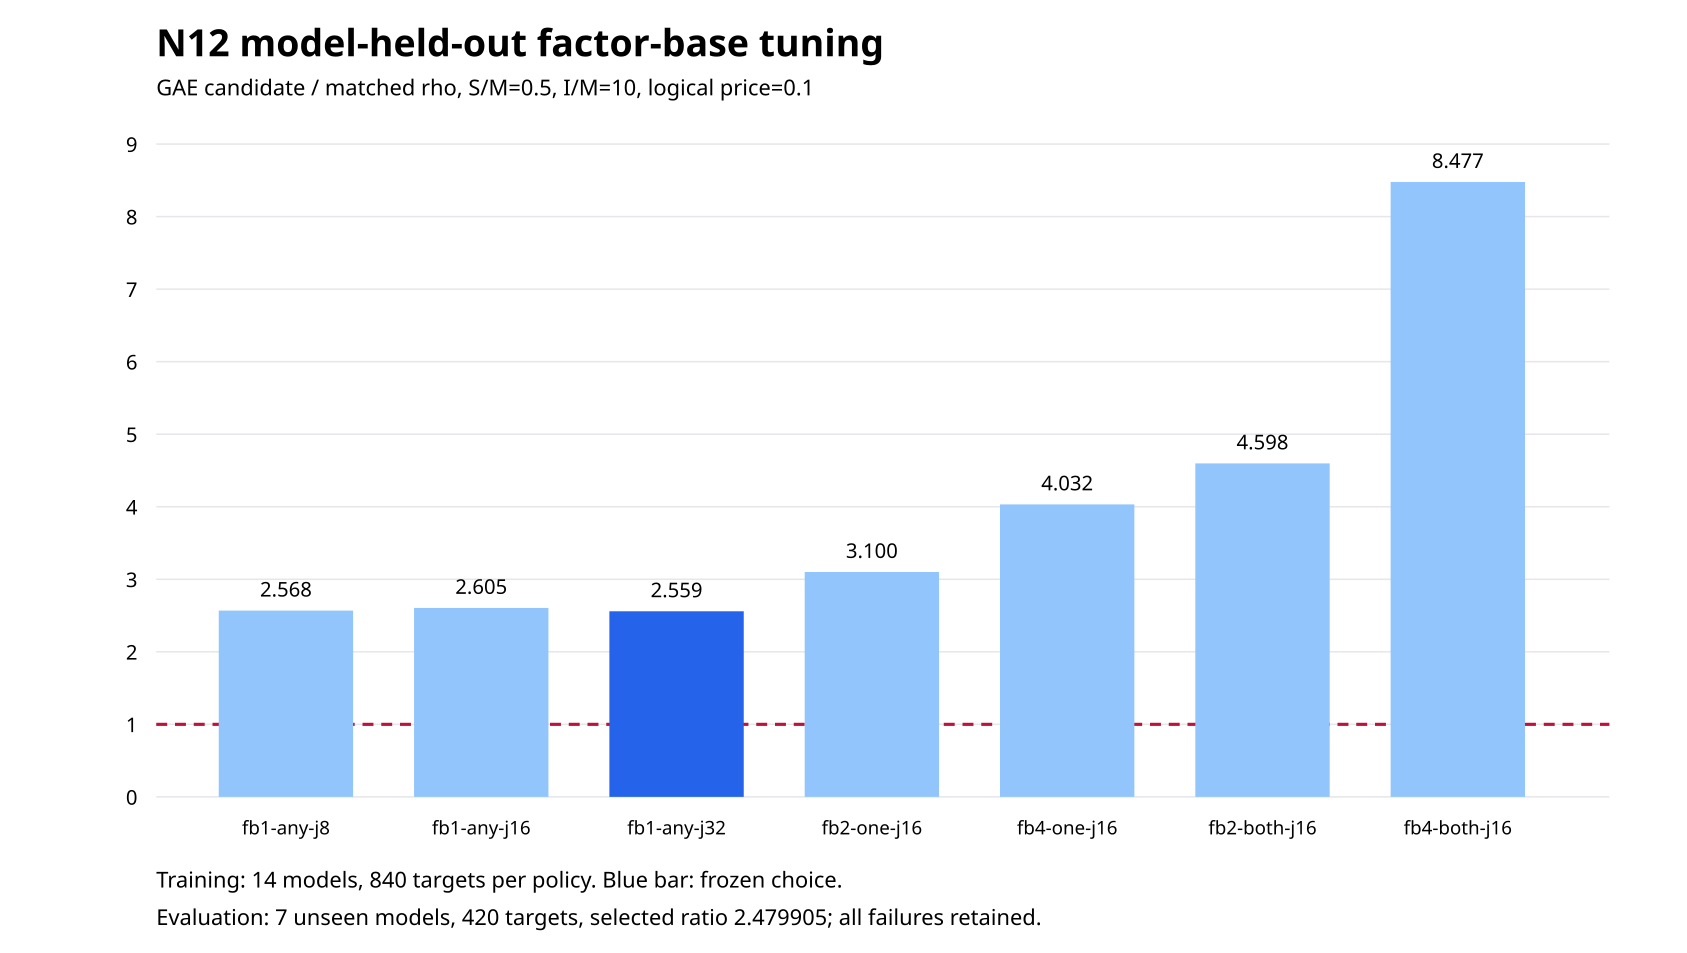
\includegraphics[width=\linewidth]{factor-base-heldout.png}
\caption{Native-analyzer representative-cell ratios for the seven training policies (840 targets each). The line at one is equal cost. The frozen evaluation ratio is printed in the graph footer.}
\end{figure}
\clearpage
\begin{figure}[h]
\centering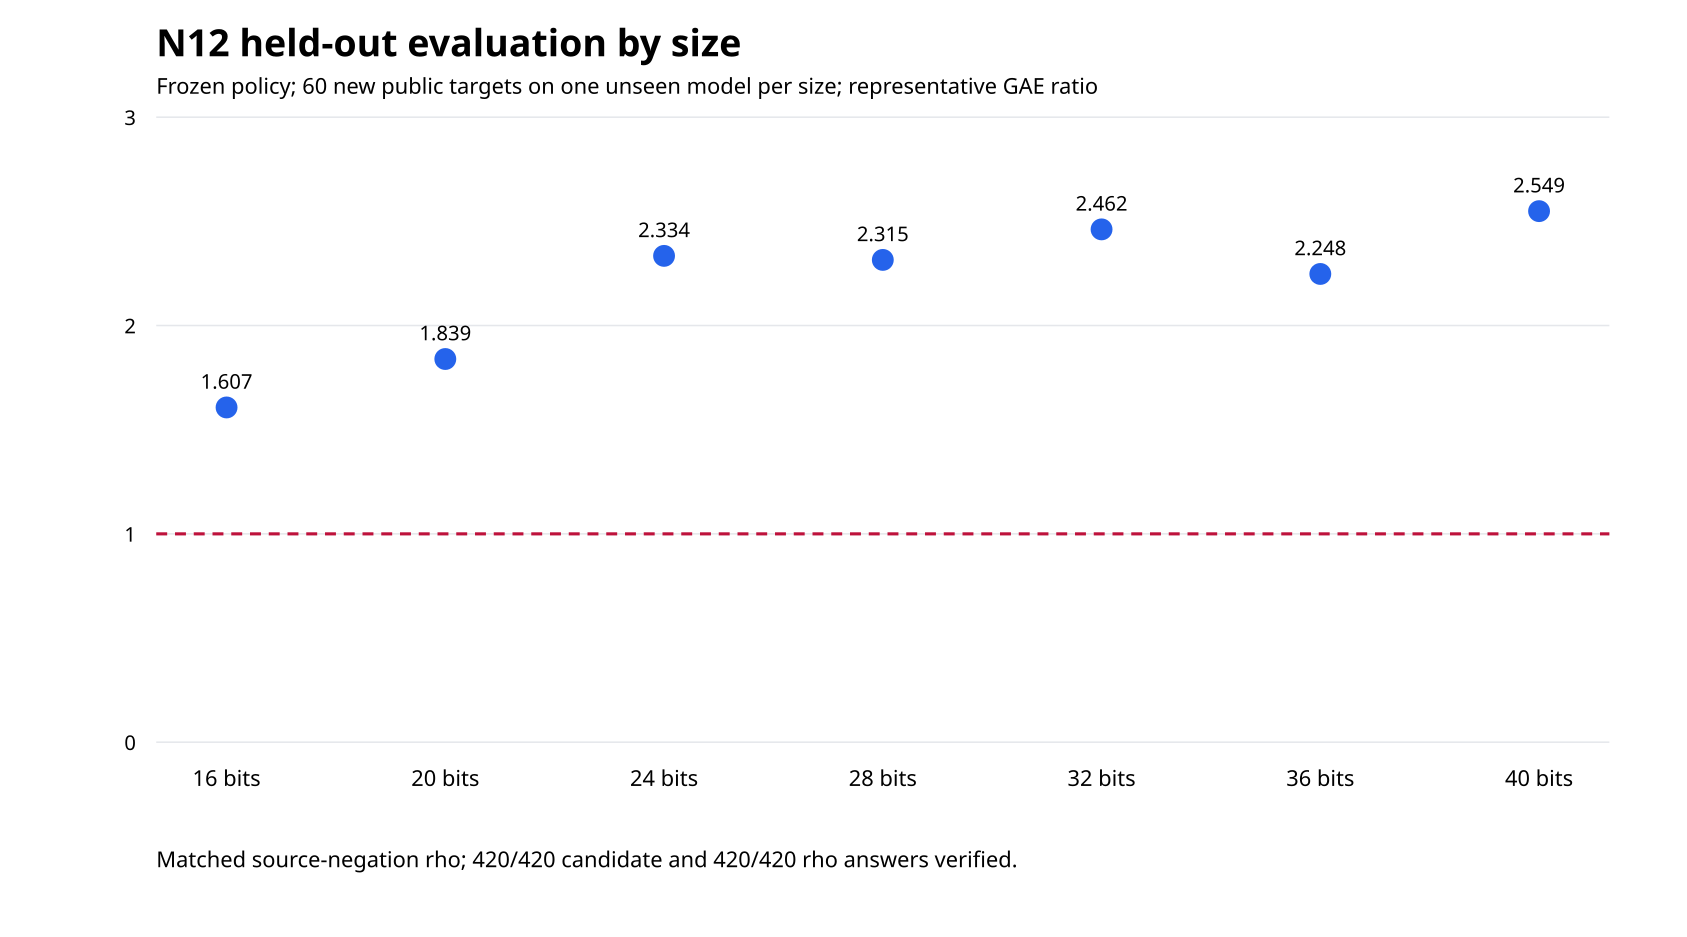
\includegraphics[width=\linewidth]{evaluation-by-size.png}
\caption{Held-out representative-cell ratio on each unseen 60-target curve model, one per size. All other prices are retained in the CSV.}
\end{figure}
\section*{Evidence and limits}
The raw records are in \texttt{results/raw/}; five reused training arms are frozen by the earlier replication artifact manifest. The standardized target files are \texttt{evaluation-targets.jsonl} and \texttt{evaluation-targets.csv}. All 36 prices for the aggregate, each model and each size are in \texttt{evaluation-price-grid.csv}; the matching training grid is \texttt{training-price-grid.csv}. The native validator independently recomputed 11760 training, 420 evaluation candidate and 420 evaluation rho source-curve scalar products, plus 252 training and 540 evaluation price cells.\par
\medskip
Every cost is a cold single-target operation count including setup and source verification. The reference is source negation rho in the same binary and process. The shared host earned no isolation tier; elapsed wall time is diagnostic and carries no speed claim. One deterministic target seed per target supplies no sampling interval. These observations are for the 21 fixed public Scholten models and this implementation; no leaderboard row is proposed.\par
\end{document}
